\section{Iteration 8: Decomposition of the Notification Unit}
\label{add:it8}

\subsection{Step 1: Identify candidate drivers}
\label{add:it8/drivers}

\npar There is only very little functionality delegated to this unit, namely one
two cases, UC9 (Notify Customer) and UCx (retrieve customer from deviceId).
Since there are no quality attributes this decomposition will be use case
driven.

\subsection{Step 2: Choose design concepts}
\label{add:it8/concepts}

\subsubsection{Tactics}
\label{add:it8/tactics}

\npar Since there are no applicable quality attributes in this iteration. There
are no tactics selected. Off course are general OO design principles such as
separation of concerns taken into account as much as possible.

\subsubsection{Design Patterns}
\label{add:it8/patterns}

\npar No patterns were found to develop the functionality of UC9.

\subsection{Step 3: Instantiate architectural elements and allocate responsibilities}
\label{add:it8/elements}

\begin{figure}[H]
	\begin{centering}
		% TODO Figure
		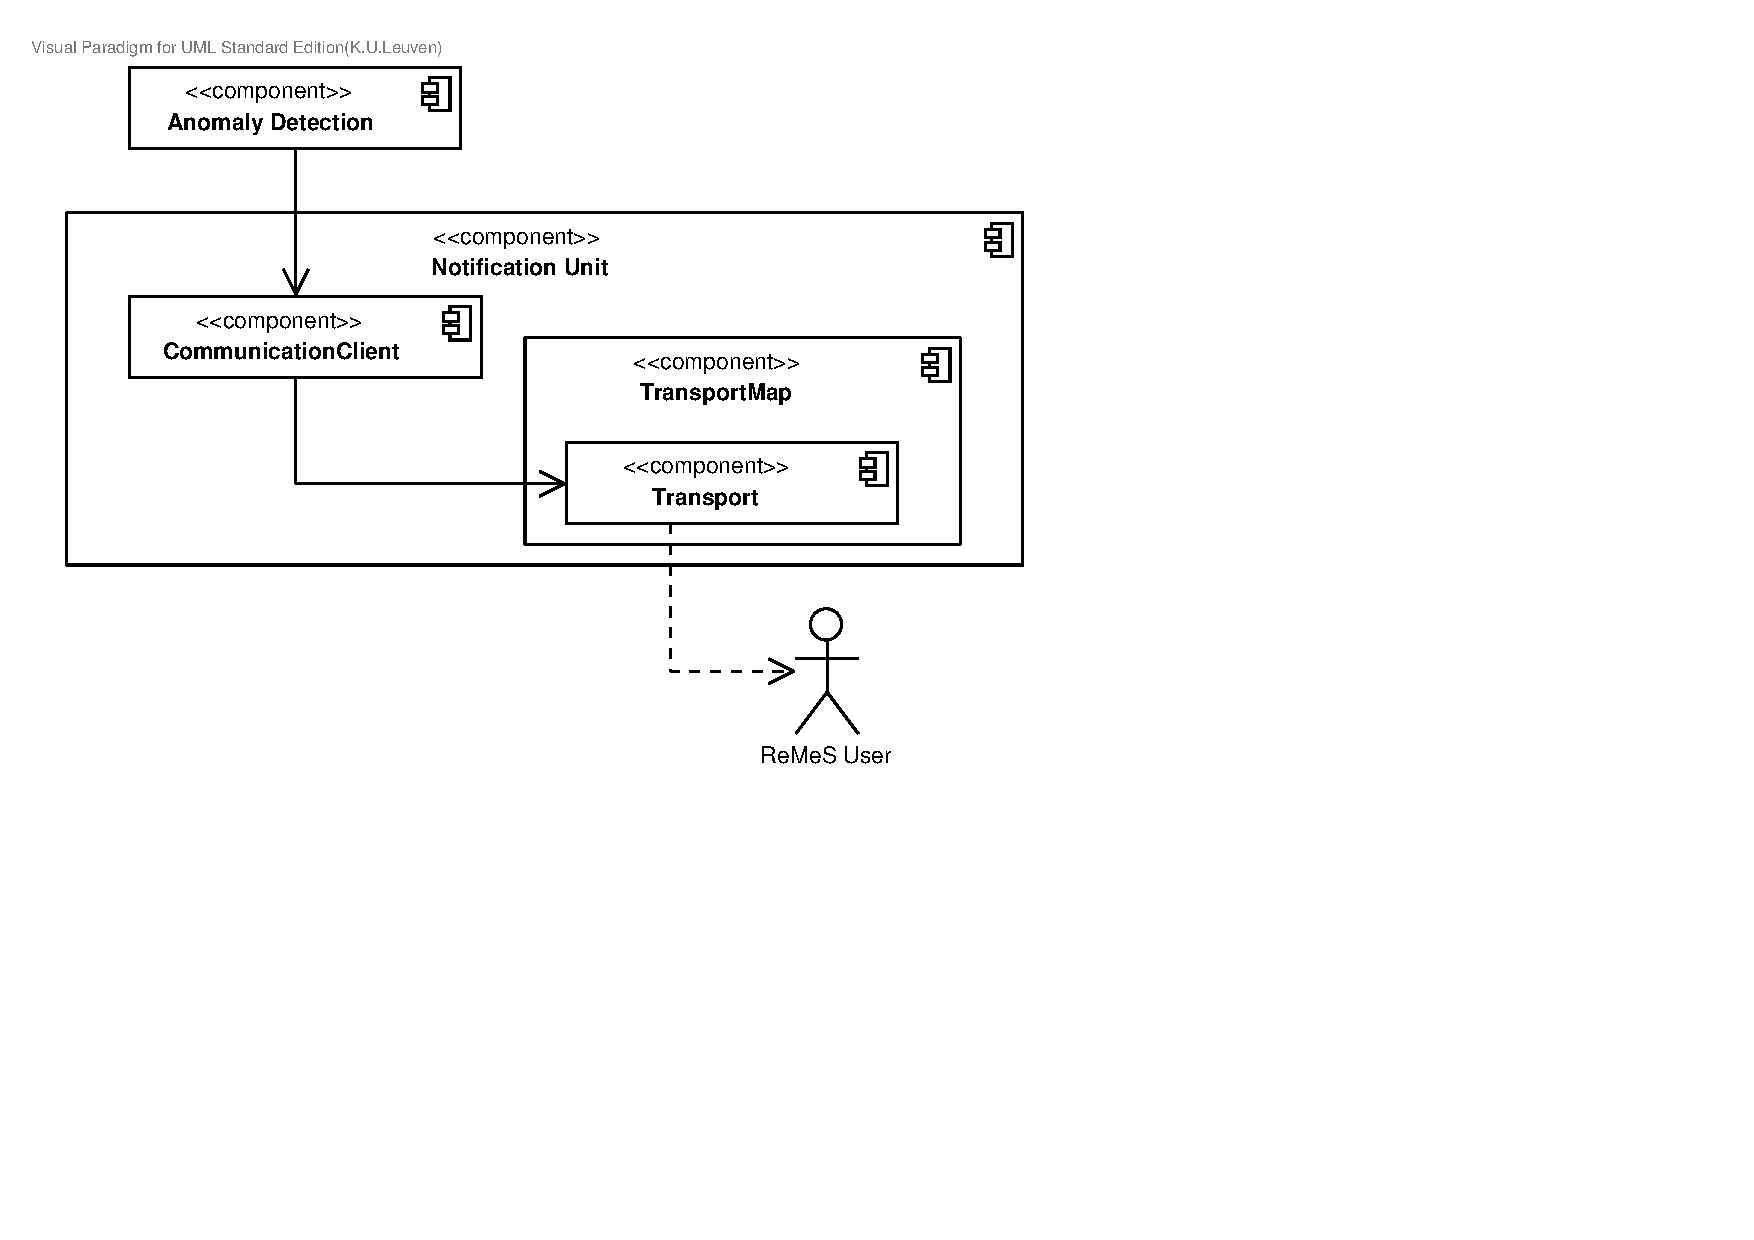
\includegraphics[width=\textwidth]{figs/add-it8-elements.pdf}
		\caption{Overview of the instantiated child elements in the Notification Unit}
		\label{fig:it8/elements}
	\end{centering}
\end{figure}

\npar There are two main components in this decomposition, the communication
client and the transport pool. Both of them will be explained below. A graphical
illustration is given in figure \ref{fig:it8/elements}.

\subsubsection{Communication Client} 
%TODO: voor de emergency services moet er misschien een shortcut voorzien worden
% ipv de overhead om nog eerst het communication channel op te zoeken ? 
\npar This component gets the initial notification message. It's task is
twofold. First of all this component has to fetch the communication channel
through which it has to contact the stakeholder (i.e. the emergency services
and/or one or more customers). Therefore it uses the \interface{CustomerProfile}
interface of the database which contains all user information. Secondly, once
the channel is acquired it has to contact the transport pool to ask for the
right transport unit which can be used to send the notification. The transport
pool offers therefore an \interface{Transport} interface.

\subsubsection{Transport Pool}

\npar The transport pool is the manager of several transport components. The
pool will return the right transport component based on the request. Each
transportcomponent is responsible for communication towards the stakeholders
through a specific channel. To realize this, each of these transport components
offers a \interface{Notify} interface. By splitting the transport into different
components the sending of notifications can be parallelized (i.e. over
different communication channels).

\subsection{Step 4: Define interfaces for instantiated elements}
\label{add:it8/interfaces}

\subsubsection{Communication Client}

\paragraph{NotifyUnit}

\npar The interface this notification unit offers, has one method, namely a
\method{send(Alarm)}. Invoking this method results in the notification of the
included recipient with the message also contains in the message parameter.

\subsubsection{Transport Pool}

\paragraph{TransportManager}

\npar The transport pool offers the \interface{Transport Manager} interface. It
contains only one method, \method{getTransport(CommunicationChannel)}. This
method has to return the right transport entity based on the
communicationChannel parameter.

\paragraph{Transport}

\npar This last interface also offers just one method, namely
\method{send(Alarm)}. Notice that this method has the same semantics as
the method of the \interface{NotifyUnit} interface, but now the communication
channel is known so the notification can physically take place.

\begin{figure}[H]
	\begin{centering}
		% TODO Figure
		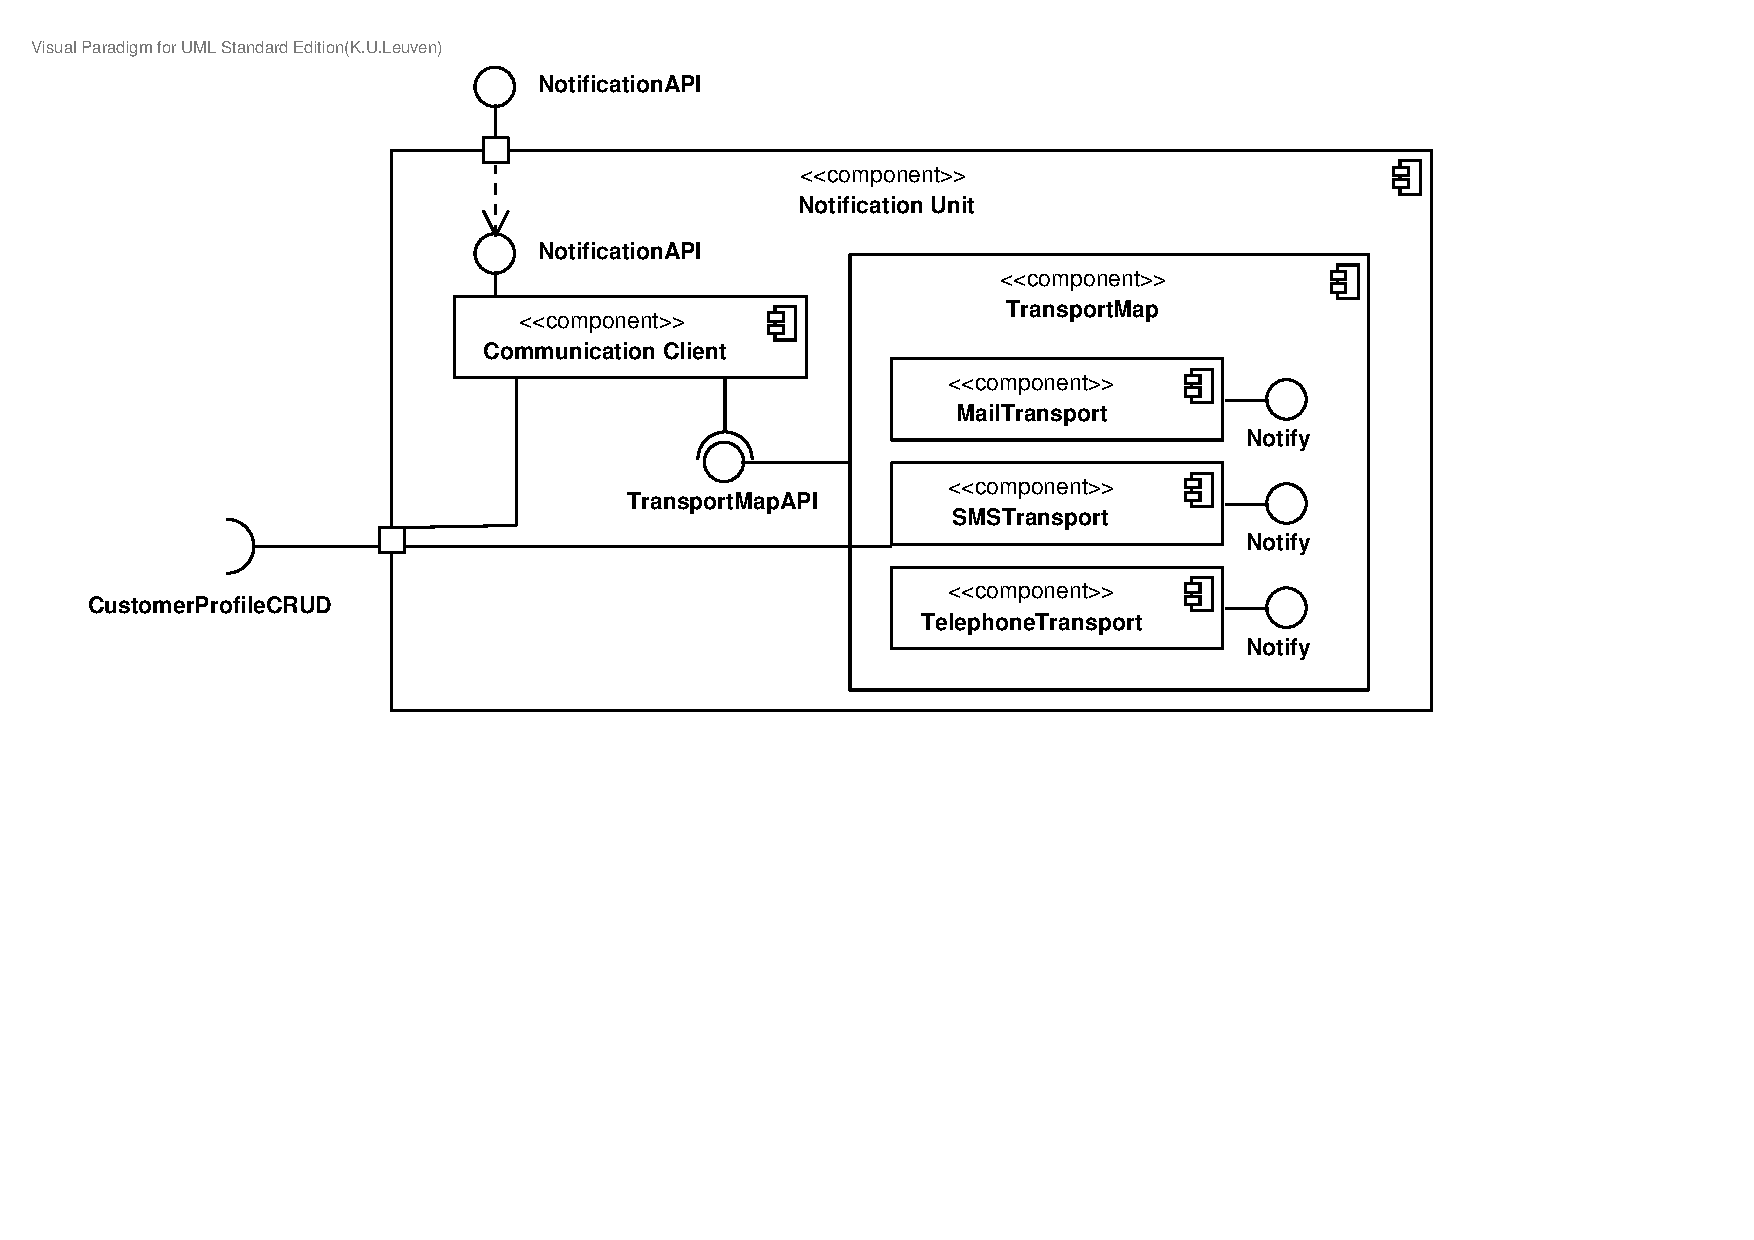
\includegraphics[width=\textwidth]{figs/add-it8-interfaces.pdf}
		\caption{Overview of the interfaces and components in the Notification Unit}
		\label{fig:it8/interfaces}
	\end{centering}
\end{figure}

\subsection{Step 5: Verify and refine}
\label{add:it8/verification}

\npar The driver of this iteration, UC9, is resolved. All the steps of its main
scenario are now tracable in the diagram.
